\chapter{Cmake}


\section{Project Structure}

See basic project and intermediate project examples, in cmake udemy.


\begin{center}
    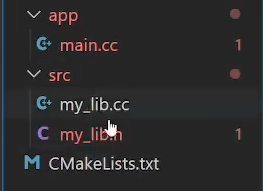
\includegraphics[width=2in]{cpp_tree1.png}
\end{center}


\begin{center}
    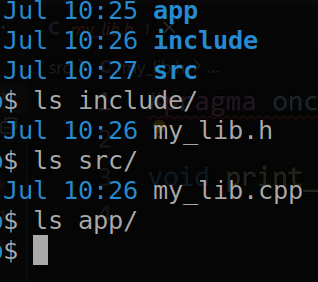
\includegraphics[width=2in]{cpp_tree2.png}
\end{center}

\section{Starter Pack - Jason Turner's Template}

\begin{verbatim}
lefticus/cmake_template // Jason Turner 2023 cmake starter pack

rename "myproject" in the cmake files to use it.
\end{verbatim}

\subsection{Lefticus Defaults - ProjectOptions.cmake}

\begin{verbatim}
Address sanitizer
Undefined behavior sanitizer
Fuzzing example built
Procedural optimization IPO (link time optimization)
Warnings as errors
Clang-tidy enabled
CPPcheck enabled
Options for precompiled headers
\end{verbatim}

\subsection{Hardening - Hardening.cmake}

\begin{verbatim}
Hardened compilation // make code safer
More compilation options / securities.

-fstack-protector
-fcf-protection
-fsanitize=undefined // undefined behavior sanitizer
-fno-sanitize-recover=undefined
-fsanitizise-minimal-runtime

+ debug information 
\end{verbatim}

\section{Simple Cmake (Modern)}

\subsection{Context}

Cmake is "a generator of make files", it abstracts away makefile complexity.

\begin{verbatim}
First, cmake // generate make files
Second, make // run make files
Last, ./hello // run the created executable
\end{verbatim}

To create an executable of hello.cpp. We usually:
\begin{verbatim}
:wq // quit vim
g++ main.cpp -o hello // compile 
./hello // run the executable
\end{verbatim}

\subsection{CMakeLists.txt}

With Cmake, we can have:

\begin{verbatim}
// have cmake installed

cmake_minimum_required(VERSION 3.10)
set(CMAKE_CXX_STANDARD 17)
set(CMAKE_CXX_STANDARD_REQUIRED ON)

project(hello VERSION 1.0)
add_executable(hello main.cpp)
\end{verbatim}

Run CMake from the command line, specify a directory.
\begin{verbatim}
cmake . && make && ./hello
\end{verbatim}

\subsection{Cmake .  }

Generates all needed make files (Artifacts).

\begin{center}
    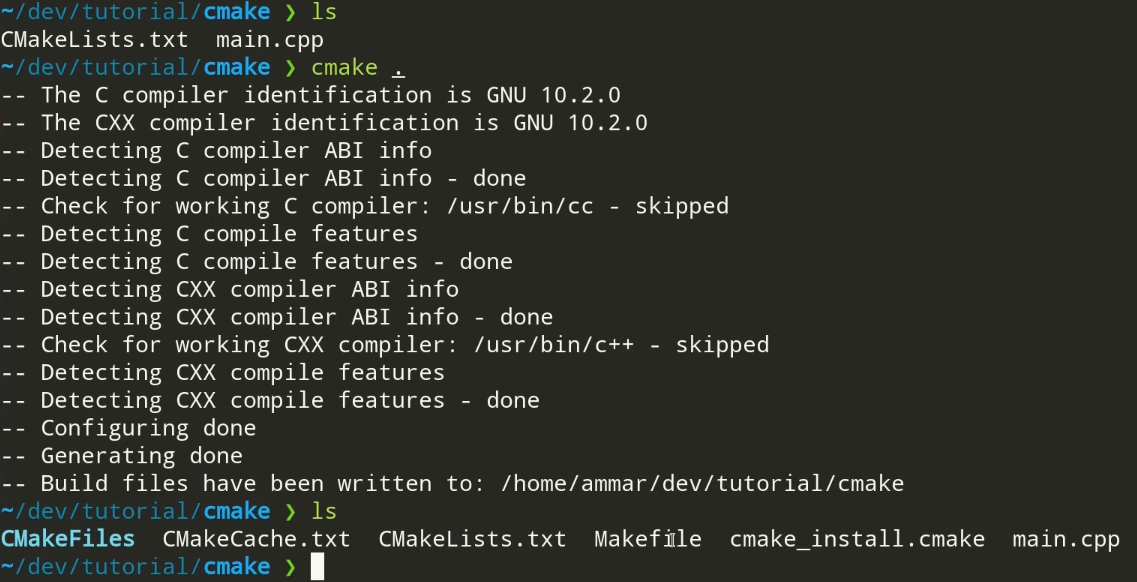
\includegraphics[width=2in]{cmake_dir.png}
\end{center}

\subsection{Make}

With the MakeFile generated by cmake. Build your binary (the executable) with:

\begin{center}
    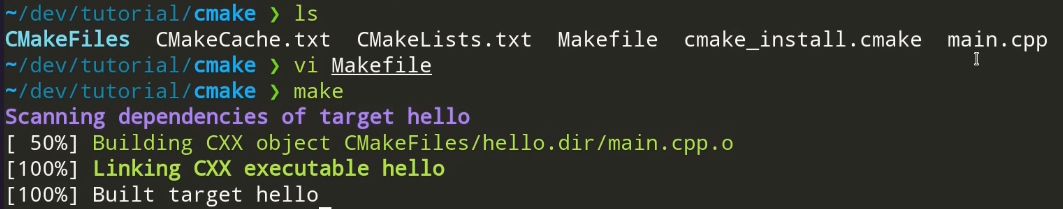
\includegraphics[width=2in]{make.png}
\end{center}

\subsection{Build folder}

\begin{center}
    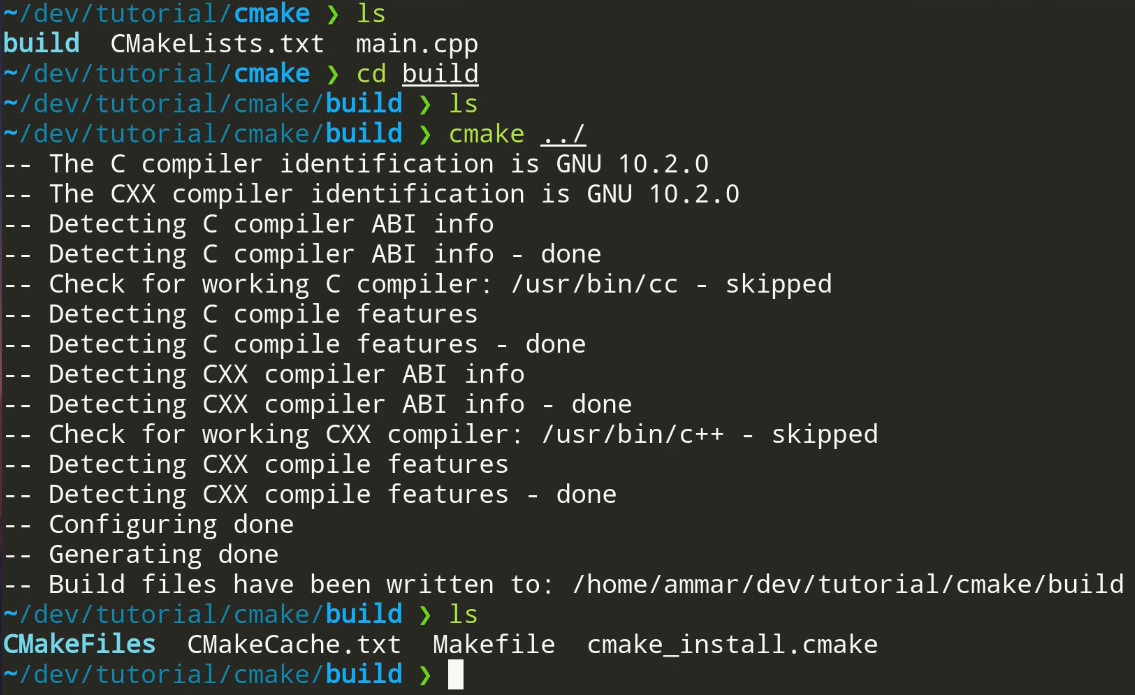
\includegraphics[width=2in]{build.png}
\end{center}

\subsection{Sick CMake Vim plugins combos}

\begin{verbatim}
See codevion/cpp2.md
\end{verbatim}

\subsection{COC - for code completion in nvim}
\begin{verbatim}
https://github.com/neoclide/coc.nvim
Jason Turner has this too
\end{verbatim}

\subsection{Include Header File - CMake Continued}

\begin{verbatim}
target_include_directories(hello PUBLIC ${CMAKE_CURRENT_SOURCE_DIR}/include)

    // Standard is having header files in /include directory!

hello // our target, where to add the stuff from headers
PUBLIC // gives the scope of added stuff from headers. 
       // Public, Private or Interface
       // Usage: when you have cmake library, make sure it is seen by #include in files

cmake_minimum_required(VERSION 3.10)
set(CMAKE_CXX_STANDARD 17)
set(CMAKE_CXX_STANDARD_REQUIRED ON)

project(hello VERSION 1.0)
add_executable(hello main.cpp)
target_include_directories(hello PUBLIC ${CMAKE_CURRENT_SOURCE_DIR}/include)
\end{verbatim}

\subsubsection{In header file}

\begin{verbatim}
#pragma once
#include <iostream>

class Blah {
    public:
        inline void boo() {
            std::cout << "Boo!\n";
        }
};
\end{verbatim}

\subsection{Pragma Once}

\begin{verbatim}
#pragma once is a non-standard directive that serves as an include guard. 
It ensures that a header file is included only once during the compilation process,
regardless of how many times it is referenced.

Placed at the beginning of a header file, it acts as a compiler directive to prevent multiple inclusions
Supported by most compilers, including GCC, Clang, and MSVC.
\end{verbatim}

\subsection{Glob - Include Many files with CMake}
 
You have at least two options. First, include every files one-by-one in the CMakeList.txt.
\begin{verbatim}
cmake_minimum_required(VERSION 3.10)
set(CMAKE_CXX_STANDARD 17)
set(CMAKE_CXX_STANDARD_REQUIRED ON)

project(hello VERSION 1.0) // traditional way to include files
add_executable(hello main.cpp Blah.cpp) // added here
target_include_directories(hello PUBLIC ${CMAKE_CURRENT_SOURCE_DIR}/include)
\end{verbatim}

Cmake discourages this glob method, but it is a more sane options for large projects.

\begin{verbatim}
file(GLOB_RECURSE SRC_FILES src/*.cpp) // glob everything in src/
add_executable(hello ${SRC_FILES})
\end{verbatim}

\subsection{/src Directory - source files}

Declaration in the header file \textbf{blah.h}.
\begin{verbatim}
#pragma once

class Blah {
    public:
        void boo(); // declaring function boo in header
}
\end{verbatim}

Definition (implementation) of class Blah in the source files \textbf{blah.cpp}.
\begin{verbatim}
#include "blah.h"
#include <iostream>

void Blah::boo() {
    std::cout << "Boo!\n"; // defining function boo in src file
}
\end{verbatim}

\textbf{In CMake - Traditionally Added}
\begin{verbatim}
add_executable(hello main.cpp src/Blah.cpp) // added here
\end{verbatim}

\textbf{In CMake - Globing}
\begin{verbatim}
file(GLOB_RECURSE SRC_FILES src/*.cpp)
add_executable(hello main.cpp ${SRC_FILES})
\end{verbatim}

\subsection{CMake Custom Libraries}

Create a lib from some source files:

\begin{verbatim}
Replace add_executable with add_library

add_library(mylib STATIC lib/blah.cpp) // create a library
                                       // Staticly linked or dynamicly linked
\end{verbatim}

Then, include it in your main executable
\begin{verbatim}
target_link_libraries(hello Public mylib)
\end{verbatim}

\subsection{Custom Library Implementation - Blah example}

\begin{center}
    
\includegraphics[width=2in]{blah_tree.png}
\end{center}

\begin{verbatim}
cmake_minimum_required(VERSION 3.10)
set(CMAKE_CXX_STANDARD 17)
set(CMAKE_CXX_STANDARD_REQUIRED ON)

project(hello VERSION 1.0)

add_library(blah STATIC blah/Blah.cpp)
target_include_directories(blah PUBLIC ${CMAKE_CURRENT_SOURCE_DIR}/blah/include)

// file(GLOB_RECURSE SRC_FILES src/*.cpp)
// now useless, since main.cpp has #include added library

// We are linking our library with our executable directly, with
// target_include_libraries

add_executable(hello main.cpp)
target_link_libraries(hello PUBLIC blah)
\end{verbatim}

The target link generates a libblah.a

\begin{center}
    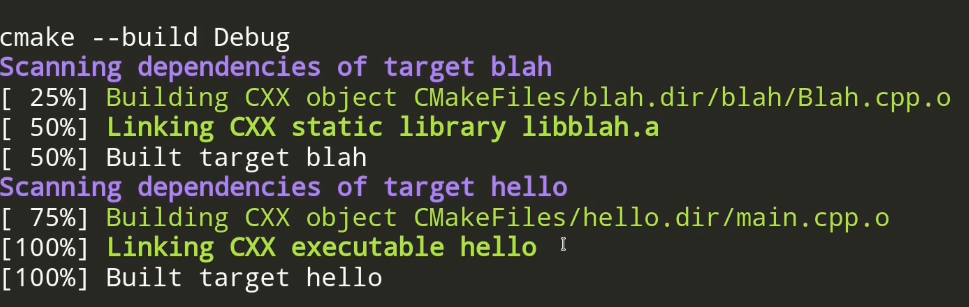
\includegraphics[width=2in]{target_link.png}
\end{center}

\section{Jason Turner's CMake Template - Options}

\begin{verbatim}
include(cmake/SystemLink.cmake)
include(cmake/LibFuzzer.cmake)
include(CMakeDependentOption)
include(CheckCXXCompilerFlag)

macro(myproject_supports_sanitizers)
  if((CMAKE_CXX_COMPILER_ID MATCHES ".*Clang.*" OR CMAKE_CXX_COMPILER_ID MATCHES ".*GNU.*") AND NOT WIN32)
    set(SUPPORTS_UBSAN ON)
  else()
    set(SUPPORTS_UBSAN OFF)
  endif()

  if((CMAKE_CXX_COMPILER_ID MATCHES ".*Clang.*" OR CMAKE_CXX_COMPILER_ID MATCHES ".*GNU.*") AND WIN32)
    set(SUPPORTS_ASAN OFF)
  else()
    set(SUPPORTS_ASAN ON)
  endif()
endmacro()

macro(myproject_setup_options)
  option(myproject_ENABLE_HARDENING "Enable hardening" ON)
  option(myproject_ENABLE_COVERAGE "Enable coverage reporting" OFF)
  cmake_dependent_option(
    myproject_ENABLE_GLOBAL_HARDENING
    "Attempt to push hardening options to built dependencies"
    ON
    myproject_ENABLE_HARDENING
    OFF)

  myproject_supports_sanitizers()

  if(NOT PROJECT_IS_TOP_LEVEL OR myproject_PACKAGING_MAINTAINER_MODE)
    option(myproject_ENABLE_IPO "Enable IPO/LTO" OFF)
    option(myproject_WARNINGS_AS_ERRORS "Treat Warnings As Errors" OFF)
    option(myproject_ENABLE_USER_LINKER "Enable user-selected linker" OFF)
    option(myproject_ENABLE_SANITIZER_ADDRESS "Enable address sanitizer" OFF)
    option(myproject_ENABLE_SANITIZER_LEAK "Enable leak sanitizer" OFF)
    option(myproject_ENABLE_SANITIZER_UNDEFINED "Enable undefined sanitizer" OFF)
    option(myproject_ENABLE_SANITIZER_THREAD "Enable thread sanitizer" OFF)
    option(myproject_ENABLE_SANITIZER_MEMORY "Enable memory sanitizer" OFF)
    option(myproject_ENABLE_UNITY_BUILD "Enable unity builds" OFF)
    option(myproject_ENABLE_CLANG_TIDY "Enable clang-tidy" OFF)
    option(myproject_ENABLE_CPPCHECK "Enable cpp-check analysis" OFF)
    option(myproject_ENABLE_PCH "Enable precompiled headers" OFF)
    option(myproject_ENABLE_CACHE "Enable ccache" OFF)
  else()
    option(myproject_ENABLE_IPO "Enable IPO/LTO" ON)
    option(myproject_WARNINGS_AS_ERRORS "Treat Warnings As Errors" ON)
    option(myproject_ENABLE_USER_LINKER "Enable user-selected linker" OFF)
    option(myproject_ENABLE_SANITIZER_ADDRESS "Enable address sanitizer" ${SUPPORTS_ASAN})
    option(myproject_ENABLE_SANITIZER_LEAK "Enable leak sanitizer" OFF)
    option(myproject_ENABLE_SANITIZER_UNDEFINED "Enable undefined sanitizer" ${SUPPORTS_UBSAN})
    option(myproject_ENABLE_SANITIZER_THREAD "Enable thread sanitizer" OFF)
    option(myproject_ENABLE_SANITIZER_MEMORY "Enable memory sanitizer" OFF)
    option(myproject_ENABLE_UNITY_BUILD "Enable unity builds" OFF)
    option(myproject_ENABLE_CLANG_TIDY "Enable clang-tidy" ON)
    option(myproject_ENABLE_CPPCHECK "Enable cpp-check analysis" ON)
    option(myproject_ENABLE_PCH "Enable precompiled headers" OFF)
    option(myproject_ENABLE_CACHE "Enable ccache" ON)
  endif()

  if(NOT PROJECT_IS_TOP_LEVEL)
    mark_as_advanced(
      myproject_ENABLE_IPO
      myproject_WARNINGS_AS_ERRORS
      myproject_ENABLE_USER_LINKER
      myproject_ENABLE_SANITIZER_ADDRESS
      myproject_ENABLE_SANITIZER_LEAK
      myproject_ENABLE_SANITIZER_UNDEFINED
      myproject_ENABLE_SANITIZER_THREAD
      myproject_ENABLE_SANITIZER_MEMORY
      myproject_ENABLE_UNITY_BUILD
      myproject_ENABLE_CLANG_TIDY
      myproject_ENABLE_CPPCHECK
      myproject_ENABLE_COVERAGE
      myproject_ENABLE_PCH
      myproject_ENABLE_CACHE)
  endif()

  myproject_check_libfuzzer_support(LIBFUZZER_SUPPORTED)
  if(LIBFUZZER_SUPPORTED AND (myproject_ENABLE_SANITIZER_ADDRESS OR myproject_ENABLE_SANITIZER_THREAD OR myproject_ENABLE_SANITIZER_UNDEFINED))
    set(DEFAULT_FUZZER ON)
  else()
    set(DEFAULT_FUZZER OFF)
  endif()

  option(myproject_BUILD_FUZZ_TESTS "Enable fuzz testing executable" ${DEFAULT_FUZZER})

endmacro()

macro(myproject_global_options)
  if(myproject_ENABLE_IPO)
    include(cmake/InterproceduralOptimization.cmake)
    myproject_enable_ipo()
  endif()

  myproject_supports_sanitizers()

  if(myproject_ENABLE_HARDENING AND myproject_ENABLE_GLOBAL_HARDENING)
    include(cmake/Hardening.cmake)
    if(NOT SUPPORTS_UBSAN 
       OR myproject_ENABLE_SANITIZER_UNDEFINED
       OR myproject_ENABLE_SANITIZER_ADDRESS
       OR myproject_ENABLE_SANITIZER_THREAD
       OR myproject_ENABLE_SANITIZER_LEAK)
      set(ENABLE_UBSAN_MINIMAL_RUNTIME FALSE)
    else()
      set(ENABLE_UBSAN_MINIMAL_RUNTIME TRUE)
    endif()
    message("${myproject_ENABLE_HARDENING} ${ENABLE_UBSAN_MINIMAL_RUNTIME} ${myproject_ENABLE_SANITIZER_UNDEFINED}")
    myproject_enable_hardening(myproject_options ON ${ENABLE_UBSAN_MINIMAL_RUNTIME})
  endif()
endmacro()

macro(myproject_local_options)
  if(PROJECT_IS_TOP_LEVEL)
    include(cmake/StandardProjectSettings.cmake)
  endif()

  add_library(myproject_warnings INTERFACE)
  add_library(myproject_options INTERFACE)

  include(cmake/CompilerWarnings.cmake)
  myproject_set_project_warnings(
    myproject_warnings
    ${myproject_WARNINGS_AS_ERRORS}
    ""
    ""
    ""
    "")

  if(myproject_ENABLE_USER_LINKER)
    include(cmake/Linker.cmake)
    configure_linker(myproject_options)
  endif()

  include(cmake/Sanitizers.cmake)
  myproject_enable_sanitizers(
    myproject_options
    ${myproject_ENABLE_SANITIZER_ADDRESS}
    ${myproject_ENABLE_SANITIZER_LEAK}
    ${myproject_ENABLE_SANITIZER_UNDEFINED}
    ${myproject_ENABLE_SANITIZER_THREAD}
    ${myproject_ENABLE_SANITIZER_MEMORY})

  set_target_properties(myproject_options PROPERTIES UNITY_BUILD ${myproject_ENABLE_UNITY_BUILD})

  if(myproject_ENABLE_PCH)
    target_precompile_headers(
      myproject_options
      INTERFACE
      <vector>
      <string>
      <utility>)
  endif()

  if(myproject_ENABLE_CACHE)
    include(cmake/Cache.cmake)
    myproject_enable_cache()
  endif()

  include(cmake/StaticAnalyzers.cmake)
  if(myproject_ENABLE_CLANG_TIDY)
    myproject_enable_clang_tidy(myproject_options ${myproject_WARNINGS_AS_ERRORS})
  endif()

  if(myproject_ENABLE_CPPCHECK)
    myproject_enable_cppcheck(${myproject_WARNINGS_AS_ERRORS} "" # override cppcheck options
    )
  endif()

  if(myproject_ENABLE_COVERAGE)
    include(cmake/Tests.cmake)
    myproject_enable_coverage(myproject_options)
  endif()

  if(myproject_WARNINGS_AS_ERRORS)
    check_cxx_compiler_flag("-Wl,--fatal-warnings" LINKER_FATAL_WARNINGS)
    if(LINKER_FATAL_WARNINGS)
      # This is not working consistently, so disabling for now
      # target_link_options(myproject_options INTERFACE -Wl,--fatal-warnings)
    endif()
  endif()

  if(myproject_ENABLE_HARDENING AND NOT myproject_ENABLE_GLOBAL_HARDENING)
    include(cmake/Hardening.cmake)
    if(NOT SUPPORTS_UBSAN 
       OR myproject_ENABLE_SANITIZER_UNDEFINED
       OR myproject_ENABLE_SANITIZER_ADDRESS
       OR myproject_ENABLE_SANITIZER_THREAD
       OR myproject_ENABLE_SANITIZER_LEAK)
      set(ENABLE_UBSAN_MINIMAL_RUNTIME FALSE)
    else()
      set(ENABLE_UBSAN_MINIMAL_RUNTIME TRUE)
    endif()
    myproject_enable_hardening(myproject_options OFF ${ENABLE_UBSAN_MINIMAL_RUNTIME})
  endif()

endmacro()
\end{verbatim}

\subsection{CPM (C++ package manager)}

\begin{verbatim}
A nice section to expand on later.
\end{verbatim}

